\documentclass[a4paper,12pt]{article}
\hbadness=10000 % prevent stupid useless warnings

\usepackage{silence}
\usepackage[utf8]{inputenc} % Supporto per caratteri UTF-8
\usepackage[T1]{fontenc} % Migliore codifica dei font
\usepackage{lmodern} % Font leggibili
\usepackage{multirow,tabularx}
\usepackage{geometry}
\usepackage{float} % La flag H nelle figure, 
\usepackage{xcolor} % Per i colori
\usepackage{hyperref} % Collegamenti ipertestuali

\hypersetup{
	colorlinks=true,
	linkcolor=blue,
	urlcolor=blue,
	pdftitle={},
	pdfauthor={},
	pdfsubject={}
}

\geometry{
  a4paper,
  total={170mm,257mm},
  left=20mm,
  top=20mm,
}
\usepackage{graphicx}
\usepackage{titling}
%\usepackage{cmbright}

\author{Umberto Frega, Leonardo Napoli}
\setlength{\headheight}{14.49998pt}
\setlength{\footskip}{47.26675pt}
\addtolength{\topmargin}{-0.49998pt}

\usepackage{fancyhdr}
\fancyhf{}
\fancyfoot[R]{
\includegraphics[width=1.5cm]{assets/logo.png}}
\fancyhead[L]{OPCal}
\fancyhead[R]{\theauthor}

\begin{document}\pagestyle{fancy}

\begin{titlepage}
	\centering
	{\Large \bfseries Progetto di MODULO 2: Laboratorio di Sistemi Informativi\par}
	{\Large Anno Accademico 2024/2025 \par}
	\vspace{1cm} % Adjust if necessary
	\vfill
	{\huge Sistema Informativo per l'Organizzazione Postale Calabrese\par}
	\vfill
	\noindent
	\begin{minipage}[t]{0.5\textwidth}
		\raggedright
		Docente \\  prof. Francesco Parisi
	\end{minipage}%
	\hfill
	\begin{minipage}[t]{0.4\textwidth}
		\raggedleft
		Studenti \\ Umberto Frega 239527 \\ Leonardo Napoli 234364
	\end{minipage}

\end{titlepage}
	\tableofcontents
	\newpage
\section{Introduzione}
L'Organizzazione Postale Calabrese (OPCal) affiliato a Poste Italiane, con sede legale a Cosenza e filiale a Rende(CS), 
consiste in un Ufficio atto alla spedizione e ricezione di corrispondenze.
\subsection{Sede}
La sede di Rende(CS) in via Marconi, 11 è una piccola struttura avente 3 sportelli e un magazzino. La sua clientela è composta 
prevalentemente da studenti della vicina Università della Calabria che effettuano operazioni di ricevimento pacchi.
La fondazione dell'ufficio risale al 2017, pertanto l'attuale sistema informativo è datato.
\subsection{Organizzativo}
Il direttore dal 2020 è il sig.Lucio Dalla. L'ufficio è diviso in 3 sezioni, la sezione Sportello con 3 dipendenti è gestita 
dal sig.Francesco de Gregori, la sezione Magazzino con 2 dipendenti è gestita dal sig.Adriano Celentano e la sezione Recapiti 
è gestita dal sig.Francesco Guccini con 2 dipendenti al suo seguito. In totale l'organizzazione ammonta a 11 dipendenti.
\begin{figure}[h]
	\centering
	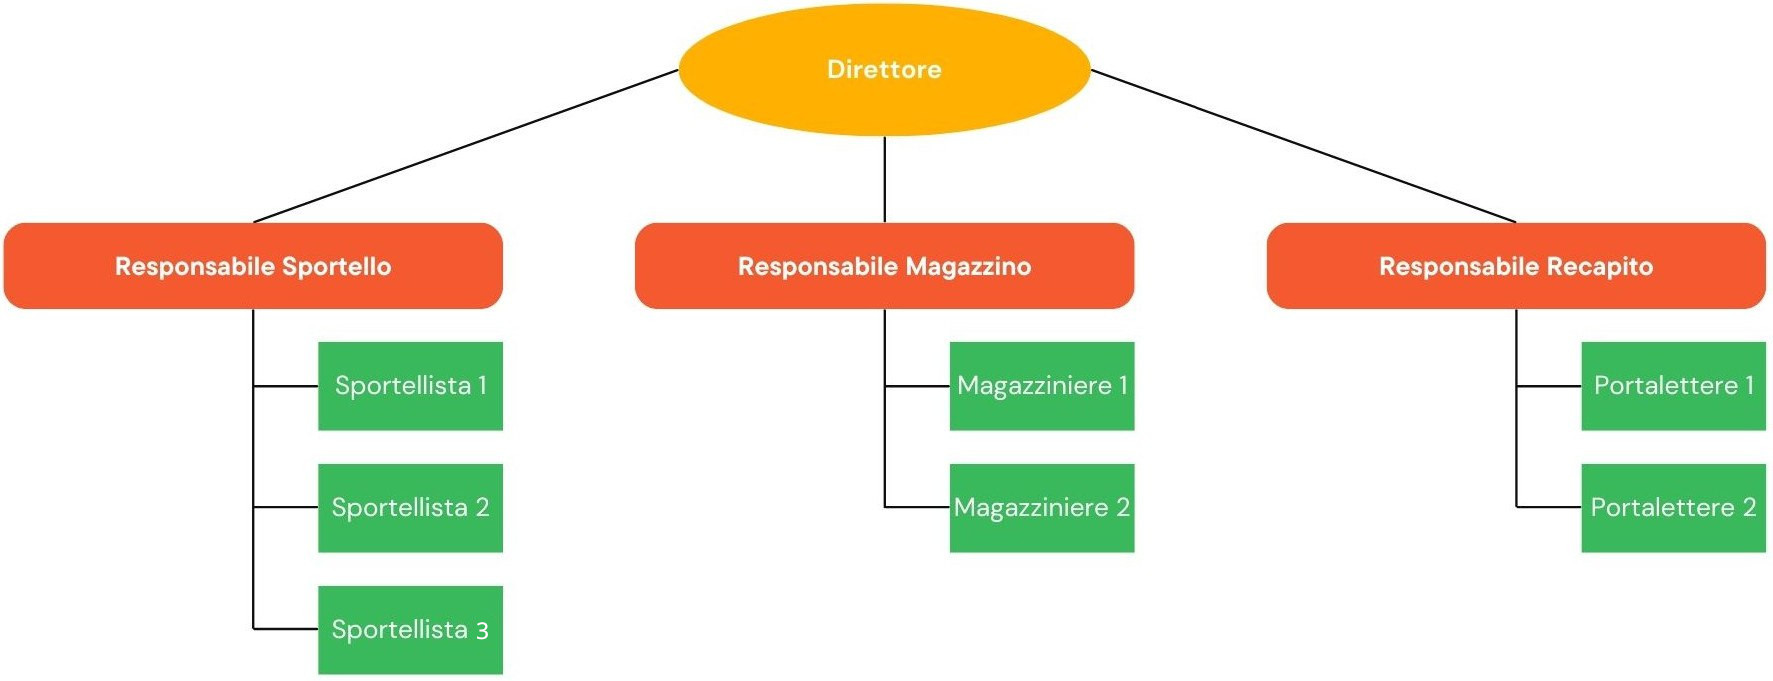
\includegraphics[width=0.8\linewidth]{assets/organigramma.jpg}
	\caption{Organigramma}
\end{figure}
\subsection{Posizione nel Mercato}
L'OPCal detiene ad oggi gran parte del palcoscenico postale cosentino, i competitor sono per la maggioranza servizi privati in rapida ascesa.
\subsection{Prospettive Future}
Nel breve termine l'obiettivo della OPCal rimane il mantenere le quote di mercato nell'area metropolitana cosentina con uno sguardo 
verso l'esterno, con la possibilità a medio/lungo termine di espandere il proprio mercato all'intera area calabrese, continuando a 
garantire una politica di serietà e velocità nel servizio e disponibilità del personale.
\subsection{Benefici Attesi}
L'implementazione del sistema all'interno dell'organizzazione aziendale porterà diversi benefici, come:
\begin{itemize}
	\item Rinnovamento del sistema attuale;
	\item Centralizzazione delle funzionalità;
	\item Centralizzazione dei dati;
	\item Rimozione della dipendenza da documenti cartacei;
	\item Maggiore possibilità di estensione dell'organizzazione;
	\item Semplificazione e deburocratizzazione della user experience;
	\item Possibilità di avere un sistema pubblicitario più esteso ed efficiente tramite il sito web;

\end{itemize}
\subsection{Funzionalità}
Le macro-funzionalità fornite dal sistema infomativo sono le seguenti:
\begin{enumerate}
	\item \textbf{Gestione dei Clienti} \begin{itemize}
		      \item Il sistema avrà la funzionalità di mantenere, organizzare e visualizzare le informazioni riguardanti i clienti, 
            quali \textit{spedizioni a carico}, \textit{saldo corrente} e \textit{pacchi in arrivo}.
		      \item Ogni cliente avrà la possibilità di visualizzare i suoi dati, prenotarsi allo sportello e prenotare una spedizione 
            tramite l'apposito sito web oppure l'applicativo per dispositivi mobile.
		      \item L'utente potrà gestire il proprio saldo corrente e decidere come utilizzarlo.
	      \end{itemize}
	\item \textbf{Gestione dei Dipendenti} \begin{itemize}
		      \item Il sistema terrà traccia dei vari dipendenti e delle operazioni che svolgono durante il giorno, nonchè dei loro 
            turni e delle loro buste paga.
		      \item Il responsabile di ciascun settore potrà visualizzare le prestazioni dei propri subordinati, allo scopo di 
            ammonire e/o premiare i dipendenti meritevoli tramite un sistema di punti.
		      \item Ogni dipendente potrà accedere alle informazioni riguardanti la propria busta paga e i turni che dovrà rispettare.
	      \end{itemize}
	\item \textbf{Gestione dei Recapiti} \begin{itemize}
		      \item Il sistema terrà traccia dello stato delle spedizioni prenotate, in corso ed effettuate in una base di dati.
		      \item La base di dati interagirà con l'interfaccia fornita ai dipendenti che si occuperanno di aggiornare lo stato 
            delle spedizioni.
		      \item Per ogni missiva presa in carico il sistema sarà responsabile di associarle un codice identificativo univoco a 
            6 cifre che contraddistinguerà l'oggetto dall'inizio alla fine della sua lavorazione,
	      \end{itemize}
	\item \textbf{Gestione del Magazzino} \begin{itemize}
		      \item Il magazzino interagirà con il sistema tramite una base di dati.
		      \item La gestione del magazzino sarà strettamente legata alla gestione dei recapiti, in quanto il magazzino contiene 
            le corrispondenze in entrata e in uscita.
		      \item Sarà possibile gestire ogni missiva tramite il codice e trovarla facilmente nonchè catalogarla in base ai suoi dati.
		      \item Per ogni oggetto nel magazzino sarà anche memorizzata la sua posizione negli scaffali.
	      \end{itemize}
	\item \textbf{Gestione Pagamenti} \begin{itemize}
		      \item Il sistema avrà la funzione di monitoraggio dei pagamenti erso l'azienda OPCal.
		      \item Il cliente potrà visualizzare lo stato dei propri pagamenti.
	      \end{itemize}
	\item \textbf{Interfaccia} \begin{itemize}
		      \item Il sistema provvede un'interfaccia per utenti e dipendenti.
		      \item Tale interfaccia avrà una duplice implementazione, un sito web e un applicativo per dispostivi mobili (Android o IOS).
		      \item Le funzionalità esposte al pubblico saranno tutte disponibili tramite le interfacce specificate,
	      \end{itemize}
\end{enumerate}

\newpage
\section{Analisi dei Requisiti}
\subsection{Analisi dello scenario}

\begin{center}
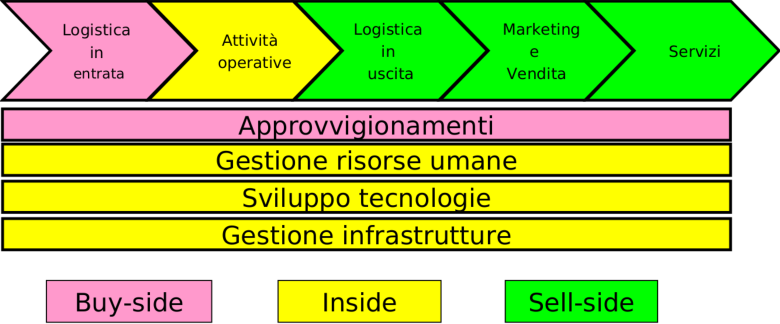
\includegraphics[width=0.8\linewidth]{assets/valueChain.png}
\vspace{1cm}

\newcolumntype{Y}{@{}>{\centering\arraybackslash}X @{}}
\newcolumntype{R}{@{}>{\raggedright\arraybackslash}X @{}}

\begin{tabularx}{\textwidth}{|*{5}{Y|}}
	\hline
  \textbf{Logistica in entrata (LE)} & \textbf{Attività operative (AO)} & \textbf{Logistica in uscita (LU)} & \textbf{Marketing e vendita (MV)} & \textbf{Servizi post-vendita (SPV)} \\ \hline

	\begin{tabular}{R}
		\hline
		LE1: registrazione cliente               \\ \hline
		LE2: aggiornamento dati cliente          \\ \hline
		LE3: registrazione operazioni dipendenti \\ \hline
		LE4: registrazione spedizioni in entrata \\ \hline
		LE5: registrazione pagamento             \\ \hline
	\end{tabular} &

	\begin{tabular}{R}
		\hline
		AO1: prenotazione spedizione  \\ \hline
		AO2: monitoraggio spedizione  \\ \hline
		AO3: modifica spedizione      \\ \hline
		AO4: supervisione prestazioni \\ \hline
		AO5: smistamento spedizioni   \\ \hline
		AO6: pagamento verso terzi    \\ \hline
  \end{tabular} &

	\begin{tabular}{R}
		\hline
		LU1: notifica spedizione \\ \hline
		LU2: consegna a cliente  \\ \hline
		LU3: consegna ricevuta   \\ \hline
	\end{tabular} &

	\begin{tabular}{R}
		\hline
		MV1: incasso allo sportello   \\ \hline
		MV2: incasso con contrassegno \\ \hline
		MV3: comunicazione promozioni \\ \hline
	\end{tabular} &

	\begin{tabular}{R}
		\hline
		SPV1: gestione resi     \\ \hline
		SPV2: gestione reclami  \\ \hline
		SPV3: raccolta feedback \\ \hline
	\end{tabular}                                                                                                                                                                    \\
	\hline

	\multicolumn{5}{|c|}{Approvvigionamenti (AP)}                                                                                                                                                       \\ \hline
	\multicolumn{5}{|c|}{AP1: acquisto consumabili}                                                                                                                                                     \\
	\multicolumn{5}{|c|}{AP2: acquisto nuova attrezzatura}                                                                                                                                              \\
	\hline
	\multicolumn{5}{|c|}{Gestione risorse umane (GRU)}                                                                                                                                                  \\ \hline
	\multicolumn{5}{|c|}{GRU1: gestione turni di lavoro}                                                                                                                                                \\
	\multicolumn{5}{|c|}{GRU2: gestione buste paga}                                                                                                                                                     \\
	\multicolumn{5}{|c|}{GRU3: valutazione dipendenti}                                                                                                                                                  \\
	\hline
	\multicolumn{5}{|c|}{Gestione infrastrutture (GI)}                                                                                                                                                  \\ \hline
	\multicolumn{5}{|c|}{GI1: manutenzione}                                                                                                                                                             \\
	\hline
\end{tabularx}
\end{center}

\newpage
\subsubsection{Registrazione cliente}
\textbf{Nome processo} (identificativo): registrazione cliente (LE1) \\
\textbf{Attori coinvolti}: Cliente, Sportellista \\
\textbf{Archivi coinvolti}: Lista degli utenti \\ 
\textbf{Descrizione del processo}:  Un \textbf{cliente} può registrarsi presentandosi in sede e richiedendo l'apposito documento da compilare con: 
nome, cognome, data di nascita e residenza, dopo di ciò lo \textbf{sportellista} inserirà il documento all'interno della \underline{lista degli utenti} 
dove all'occorrenza inserirà anche i dati in merito alle sue spedizioni (vedi LE4: registrazioni spedizioni in entrata). Nel caso in cui il \textbf{cliente} 
volesse accedere ai suoi dati si deve recare in sede e richiederle allo \textbf{sportellista}, che attingerà alla \underline{lista degli utenti}, questi dati 
sono sempre aggiornati dagli \textbf{sportellisti} (vedi LE2: aggiornamento dati cliente). \\ \\
\textbf{Processi correlati:}\\LE2,LE4.\\ \newline
\underline{Cosiderazioni dopo l'implementazione del nuovo sistema informativo}: \\ Queste operazioni saranno gestite in automatico tramite l'apposita piattaforma, 
senza che il cliente vada in sede e senza che lo sportellista lo inserisca manualmente nell'archivio.
\begin{figure}[H]
	\centering
	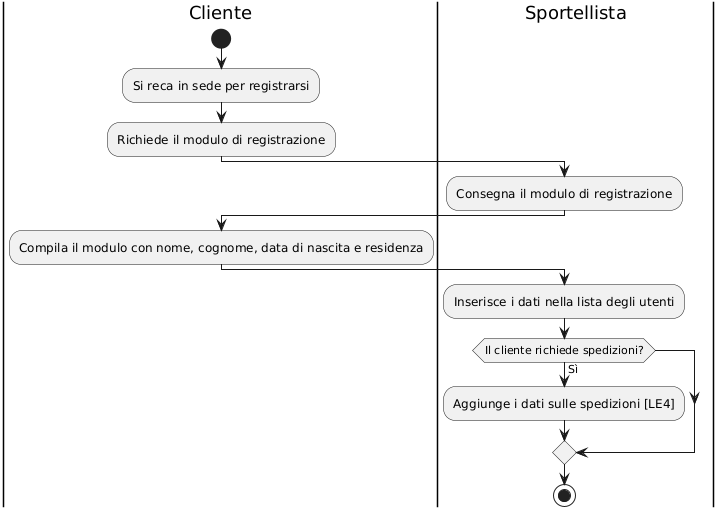
\includegraphics[width=0.8\linewidth]{assets/activitydiagram_LE1.png}
	\caption{Activity Diagram per LE1}
\end{figure}

\end{document}
